%%%%%%%%%%%%%%%%%%%%%%%%%%%%%%%%%%%%%%%%%%%%%%%%%%
%
% JSNS2 nanopulser optical calibration system manual
% 2019.03.18 s.j.m.peeters@sussex.ac.uk
%
%%%%%%%%%%%%%%%%%%%%%%%%%%%%%%%%%%%%%%%%%%%%%%%%%%
\documentclass[fleqn,10pt]{wlscirep}

%%%%%%%%%%%%%%%%%%%%%%%%%%%%%%%%%%%%%%%%%%%%%%%%%%
% IF STATEMENTS (DRAFT,..)
%%%%%%%%%%%%%%%%%%%%%%%%%%%%%%%%%%%%%%%%%%%%%%%%%%

\newif\ifdraft
%\draftfalse
\drafttrue

%%%%%%%%%%%%%%%%%%%%%%%%%%%%%%%%%%%%%%%%%%%%%%%%%%
% PACKAGE IMPORTS
%%%%%%%%%%%%%%%%%%%%%%%%%%%%%%%%%%%%%%%%%%%%%%%%%%
\usepackage[utf8]{inputenc}
\usepackage[T1]{fontenc}   
\usepackage{pdfpages}
\usepackage{amssymb} % more options for symbols (can also add amsmath/amstext)
\usepackage{etoolbox} % toggle options (e.g. names of people on/off)
\usepackage{expl3} % code for lookahead functionality of latin abbrev.
\usepackage{graphicx,subfigure} % place images
\usepackage{ifthen} % for definitions of edit and comment macros
\usepackage{isotope}
\usepackage[normalem]{ulem} % for reviewer macros, underline text etc.
\usepackage{siunitx}
\usepackage{xargs}
\usepackage{xspace} % for dynamic spaces (e.g. none before a colon, ...)

\ifdraft
%\usepackage{draftwatermark} % set watermark
\usepackage{lineno} % line numbers
\usepackage[colorinlistoftodos,prependcaption,textsize=tiny]{todonotes}
\fi

%%%%%%%%%%%%%%%%%%%%%%%%%%%%%%%%%%%%%%%%%%%%%%%%%%
% Commonly used words
%%%%%%%%%%%%%%%%%%%%%%%%%%%%%%%%%%%%%%%%%%%%%%%%%%
\newcommand*{\jsns}{JSNS\textsuperscript{2}\xspace}

%%%%%%%%%%%%%%%%%%%%%%%%%%%%%%%%%%%%%%%%%%%%%%%%%%
% Todo notes
%%%%%%%%%%%%%%%%%%%%%%%%%%%%%%%%%%%%%%%%%%%%%%%%%%
\newcommandx{\missing}[2][1=]{\ifdraft \todo[linecolor=red,backgroundcolor=red!25,bordercolor=black,#1]{#2} \fi}
\newcommandx{\fix}[2][1=]{\ifdraft \todo[linecolor=yellow,backgroundcolor=yellow!25,bordercolor=black,#1]{#2} \fi}
\newcommandx{\info}[2][1=]{\ifdraft \todo[linecolor=green,backgroundcolor=green!25,bordercolor=black,#1]{#2} \fi}

%%%%%%%%%%%%%%%%%%%%%%%%%%%%%%%%%%%%%%%%%%%%%%%%%%
% Set watermark and linenumbers
%%%%%%%%%%%%%%%%%%%%%%%%%%%%%%%%%%%%%%%%%%%%%%%%%%
\ifdraft
 %\SetWatermarkText{DRAFT}
 %\SetWatermarkScale{1.0}
 \linenumbers
\fi

%%%%%%%%%%%%%%%%%%%%%%%%%%%%%%%%%%%%%%%%%%%%%%%%%%
% Title and authors
%%%%%%%%%%%%%%%%%%%%%%%%%%%%%%%%%%%%%%%%%%%%%%%%%%

\title{\jsns nanopulser optical calibration system}

\author[1]{H. Furuta}
\author[3]{A. Gibson}
\author[1]{Y. Hino}
\author[2]{Tsunayuki Matsubara}
\author[3,*]{S. J.M.~Peeters}
\author[3]{J.~Waterfield}
\author[3]{Richard~White}
\affil[1]{Tohoku University, Japan}
\affil[2]{Tokyo Metropolitan University, Japan}
\affil[3]{University of Sussex, University of Sussex}
\affil[*]{Corresponding author: s.j.m.peeters@sussex.ac.uk}

%%%%%%%%%%%%%%%%%%%%%%%%%%%%%%%%%%%%%%%%%%%%%%%%%%
% Abstract
%%%%%%%%%%%%%%%%%%%%%%%%%%%%%%%%%%%%%%%%%%%%%%%%%%

\begin{abstract}
This note describes the the \jsns nanopulser optical calibration system. The document discusses the requirements, design, testing, as well as the control software and the operation. This is a live document and should be updated as the system expands\cite{GITHUB_DOC}.
\end{abstract}

%%%%%%%%%%%%%%%%%%%%%%%%%%%%%%%%%%%%%%%%%%%%%%%%%%
% Begin document
%%%%%%%%%%%%%%%%%%%%%%%%%%%%%%%%%%%%%%%%%%%%%%%%%%

\begin{document}

\flushbottom
\maketitle

{\raggedright\sffamily\bfseries\fontsize{12}{14}\selectfont Version: \date{\today}}


\thispagestyle{empty}

%%%%%%%%%%%%%%%%%%%%%%%%%%%%%%%%%%%%%%%%%%%%%%%%%%
% Introduction
%%%%%%%%%%%%%%%%%%%%%%%%%%%%%%%%%%%%%%%%%%%%%%%%%%

\section*{Introduction}
% !TeX root = 00main.tex

%%%%%%%%%%%%%%%%%%%%%%%%%%%%%%%%%%%%%%%%%%%%%%%%%%%%%%%%%%%%%%%%%%%%%%%%%%%
% Introduction
%%%%%%%%%%%%%%%%%%%%%%%%%%%%%%%%%%%%%%%%%%%%%%%%%%%%%%%%%%%%%%%%%%%%%%%%%%%

The \jsns experiment\cite{JSNS2TDR} is a relatively small liquid scintillator detector. It relies on precise timing in order to seperate the scintillation light from Cherenkov light, which is crucial for background and signal separation. This note describes the \jsns2 nanopulser optical calibration system that will be used to do the timing calibration, as well as the gain calibration.

We start with a description of the requirements as set by the \jsns collaboration. Next is a description of the system in the experiment. We then describe the control software, followed by a section on the analysis strategy.

This document is maintained by the corresponding author and can be dowloaded or cloned from github\cite{GITHUB_DOC}.

\fix[inline]{SJMP: Expand introduction}


%%%%%%%%%%%%%%%%%%%%%%%%%%%%%%%%%%%%%%%%%%%%%%%%%%
% Requirements
%%%%%%%%%%%%%%%%%%%%%%%%%%%%%%%%%%%%%%%%%%%%%%%%%%

\section*{Requirements}
% !TeX root = 00main.tex

%%%%%%%%%%%%%%%%%%%%%%%%%%%%%%%%%%%%%%%%%%%%%%%%%%%%%%%%%%%%%%%%%%%%%%%%%%%
% Requirements
%%%%%%%%%%%%%%%%%%%%%%%%%%%%%%%%%%%%%%%%%%%%%%%%%%%%%%%%%%%%%%%%%%%%%%%%%%%

The calibration system has the following requirements:

\begin{enumerate}
\item The system is controllable via simple to use, and flexible software.\\ 
\emph{This is what we provided.} \missing[inline]{SJMP: fill \& add reference}
\item The part of the system that is inside the LAB filled volume is compatible with LAB.\\ 
\emph{This is what we provided.} \missing[inline]{SJMP: fill \& add reference}
\item The system does not cause interference on the PMT array.\\ 
\emph{This is what we provided.} \missing[inline]{SJMP: fill \& add reference}
\item Each pulser produces a very small width in time optical pulse (less than 1 ns risetime at low intensities and less than 2 ns falltime).\\ 
\emph{This is what we provided.} \missing[inline]{SJMP: fill \& add reference}
\item The system provides full optical coverage of the PMT array for both 420~nm and 355~nm.\\ 
\emph{This is what we provided.} \missing[inline]{SJMP: fill \& add reference}
\item The system provides a trigger pulse that can be delayed, with negative amplitude and less than 1 1~V, to be read-out with one channel of the VX1721 flash ADC read-out system.\\ 
\emph{This is what we provided.}\missing[inline]{SJMP: fill \& add reference}
\end{enumerate}

%%%%%%%%%%%%%%%%%%%%%%%%%%%%%%%%%%%%%%%%%%%%%%%%%%
% System design
%%%%%%%%%%%%%%%%%%%%%%%%%%%%%%%%%%%%%%%%%%%%%%%%%%

\section*{System design}
\input design

%%%%%%%%%%%%%%%%%%%%%%%%%%%%%%%%%%%%%%%%%%%%%%%%%%
% System commissioning
%%%%%%%%%%%%%%%%%%%%%%%%%%%%%%%%%%%%%%%%%%%%%%%%%%

\section*{System commissioning}
% !TeX root = 00main.tex

%%%%%%%%%%%%%%%%%%%%%%%%%%%%%%%%%%%%%%%%%%%%%%%%%%
% System commissioning
%%%%%%%%%%%%%%%%%%%%%%%%%%%%%%%%%%%%%%%%%%%%%%%%%%

\subsection*{Commissioning at the University of Sussex}

\subsubsection*{Initial commissioning}

The nanopulser optical calibration system (serial nr OP\_12\_420\_2\_355) has been tested at the University of Sussex in February 2019, and the results of this are shown in Table~\ref{table:sussex_commissioning}.

The system was then shipped to Japan and tested again for functionality at the \jsns lab in the KEK building at J-PARC. The system was found to be working as expected, expect for pulserhead 7. This was replaced with a spare one (programmed to reflect the position), which worked correctly.

\begin{table}[h!]
  \begin{center}
    \caption{Results of the commissioning at the University of Sussex. The measurements are only relative: settings indicated are for which the trigger pulser and the light pulse were observed at the same time, using the specific test set-up at Sussex. The amplitude was as measured with a Hamatsu mini-PMT with mylar filter using the maximum light output setting. Note that the quantum efficiency for the UV LEDs, pulserheads 2 and 13, is much lower.}
    \label{table:sussex_commissioning}
    \begin{tabular}{|c|c|c|c|c|c|c|c|c|c|c|c|c|} 
	\hline
	 & \multicolumn{4}{c|}{LED1} & \multicolumn{4}{c|}{LED2} & \multicolumn{4}{c|}{LED3} \\
	\cline{2-13}
		        & Pulser & Trigger  & Fibre  & Amp.
		        & Pulser & Trigger  & Fibre  & Amp.
		        & Pulser & Trigger  & Fibre  & Amp. \\
	              & head    & delay & length & (V) 
			 & head    & delay & length & (V) 
                    & head    & delay & length & (V) \\
	Branch    & & & delay & & & & delay & & & & delay & \\
	             & & (ns) & (ns) & & & (ns) & (ns) & & & (ns) & (ns) & \\
       \hline 
	1 & 1 & 810 & 21 & 2.7 & 2 & 830 & 18 & 1.1 & 3 & 815 & 7 & 1.8 \\
	2 & 4 & 795 & 7  & 3.5 & 5 & 810 & 19 & 5.0 & & & & \\
	3 & 6 & 810 & 19 & 3.3 & 7 & 815 & 12 & 3.5 & & & & \\
	4 & 8 & 800 & 32 & 5.0 & 9 & 850 & 8 & 3.0 & & & & \\
	5 & 10 & 825 & 0 & 3.0 & 11 & 835 & 11 & 4.0 & & & & \\
	6 & 12 & 830 & 17 & 1.5 & 13 & 830 & 2 & 0.5 & 14 & 850 & 4 & 2.5 \\
	\hline
    \end{tabular}
  \end{center}
\end{table}

\subsubsection*{Further commissioning}

The following tasks still remain for commissioning:
\begin{itemize}
\item Estimate the delay needed for the system once installed.
\item Confirm the settings of Table~\ref{table:sussex_commissioning} and find the values for the estimated delay between optical pulse and the trigger. Try to get the all channels as close as possible. Note the (estimated) magnitude of (any) trigger jitter, if observed.
\item Find the optical range for each channel - the minimal pulse is around pulse height setting 10,000. Find the actual minimal value and note the pulse integral observed in the PMT used, as well as the pulse integral when using the maximum value pulse height setting.
\end{itemize}

\subsubsection*{Analysis methods}

The calibration of the system is done in the lab. Experience shows, that once installed in the experiment, things change - generally both due to changes in the system as well as due to different routing and noise environment. Therefore, the system will need to be recalibrated, or at least verified in analysis.

The following tasks are envisaged:
\begin{itemize}
\item 
\item
\item 
\end{itemize}

%%%%%%%%%%%%%%%%%%%%%%%%%%%%%%%%%%%%%%%%%%%%%%%%%%
% Bibliography
%%%%%%%%%%%%%%%%%%%%%%%%%%%%%%%%%%%%%%%%%%%%%%%%%%
\newpage
\bibliography{nanopulser}

%%%%%%%%%%%%%%%%%%%%%%%%%%%%%%%%%%%%%%%%%%%%%%%%%%
% Appendices
%%%%%%%%%%%%%%%%%%%%%%%%%%%%%%%%%%%%%%%%%%%%%%%%%%

\newpage
\appendix
% !TeX root = 00main.tex

%%%%%%%%%%%%%%%%%%%%%%%%%%%%%%%%%%%%%%%%%%%%%%%%%%%%%%%%%%%%%%%%%%%%%%%%%%%
% Appendices
%%%%%%%%%%%%%%%%%%%%%%%%%%%%%%%%%%%%%%%%%%%%%%%%%%%%%%%%%%%%%%%%%%%%%%%%%%%

\fix[inline]{AG: check drawings}
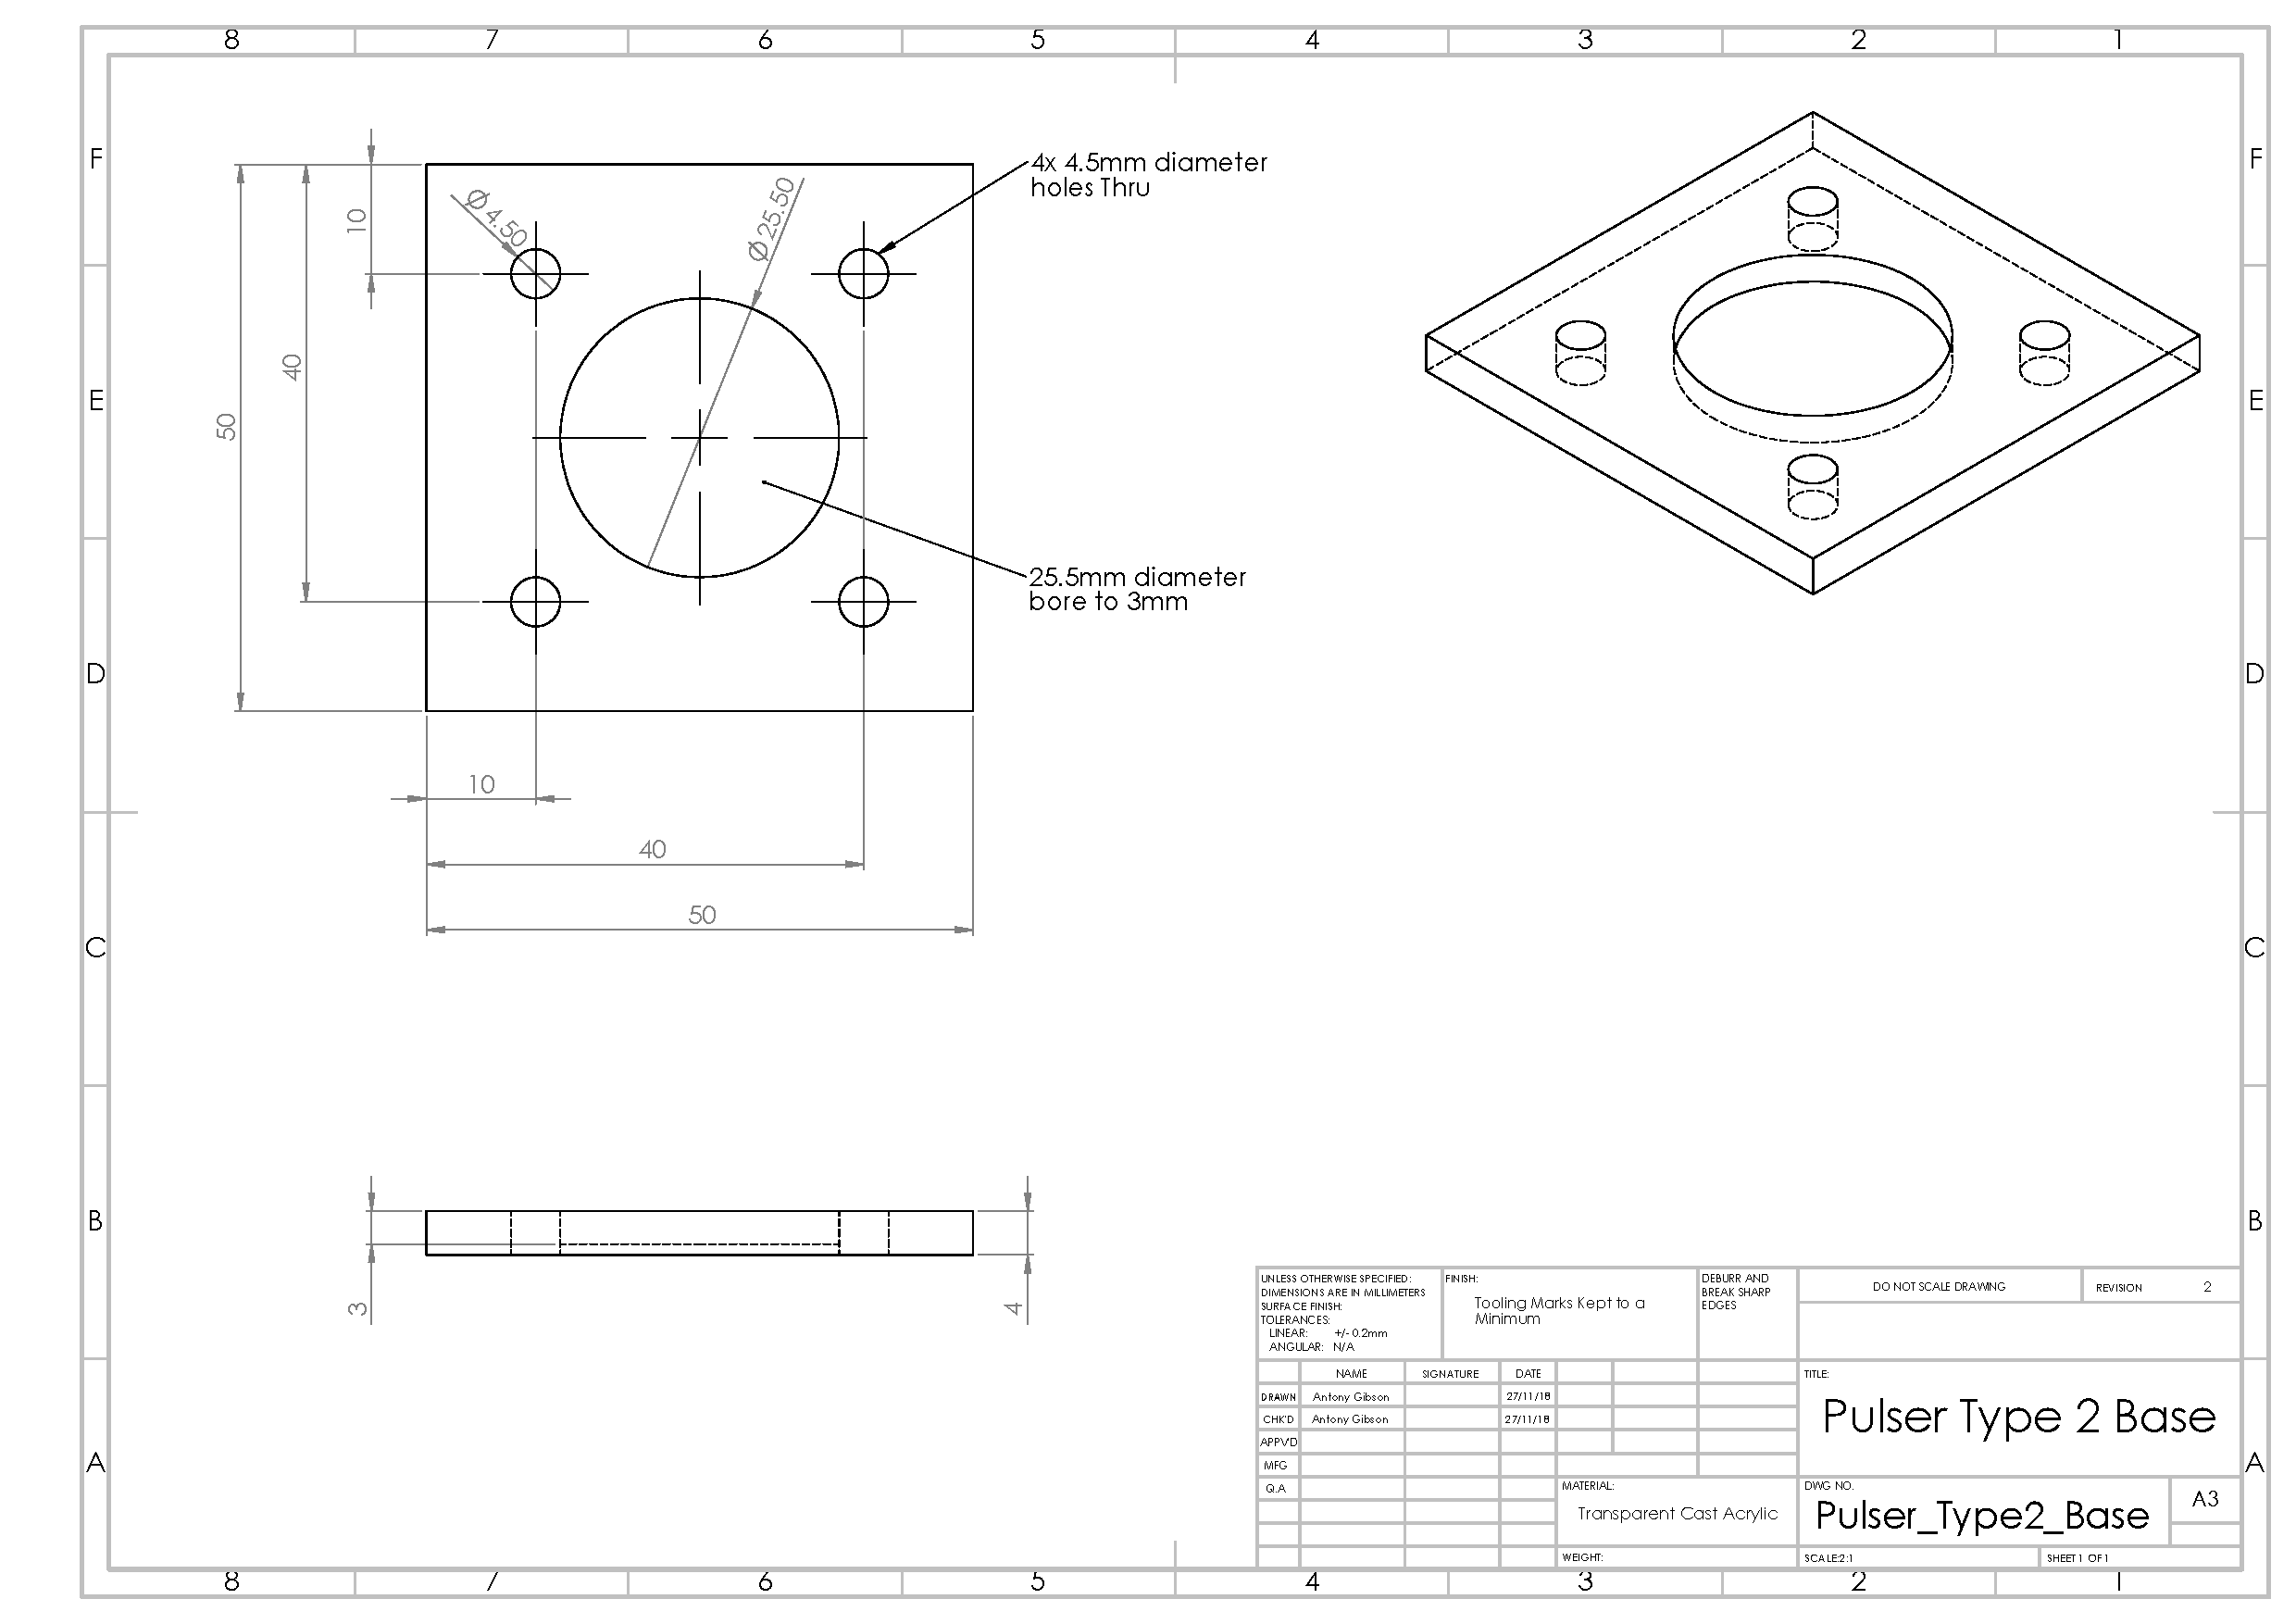
\includepdf{figures/Pulser_Type2_Base_V2.PDF}
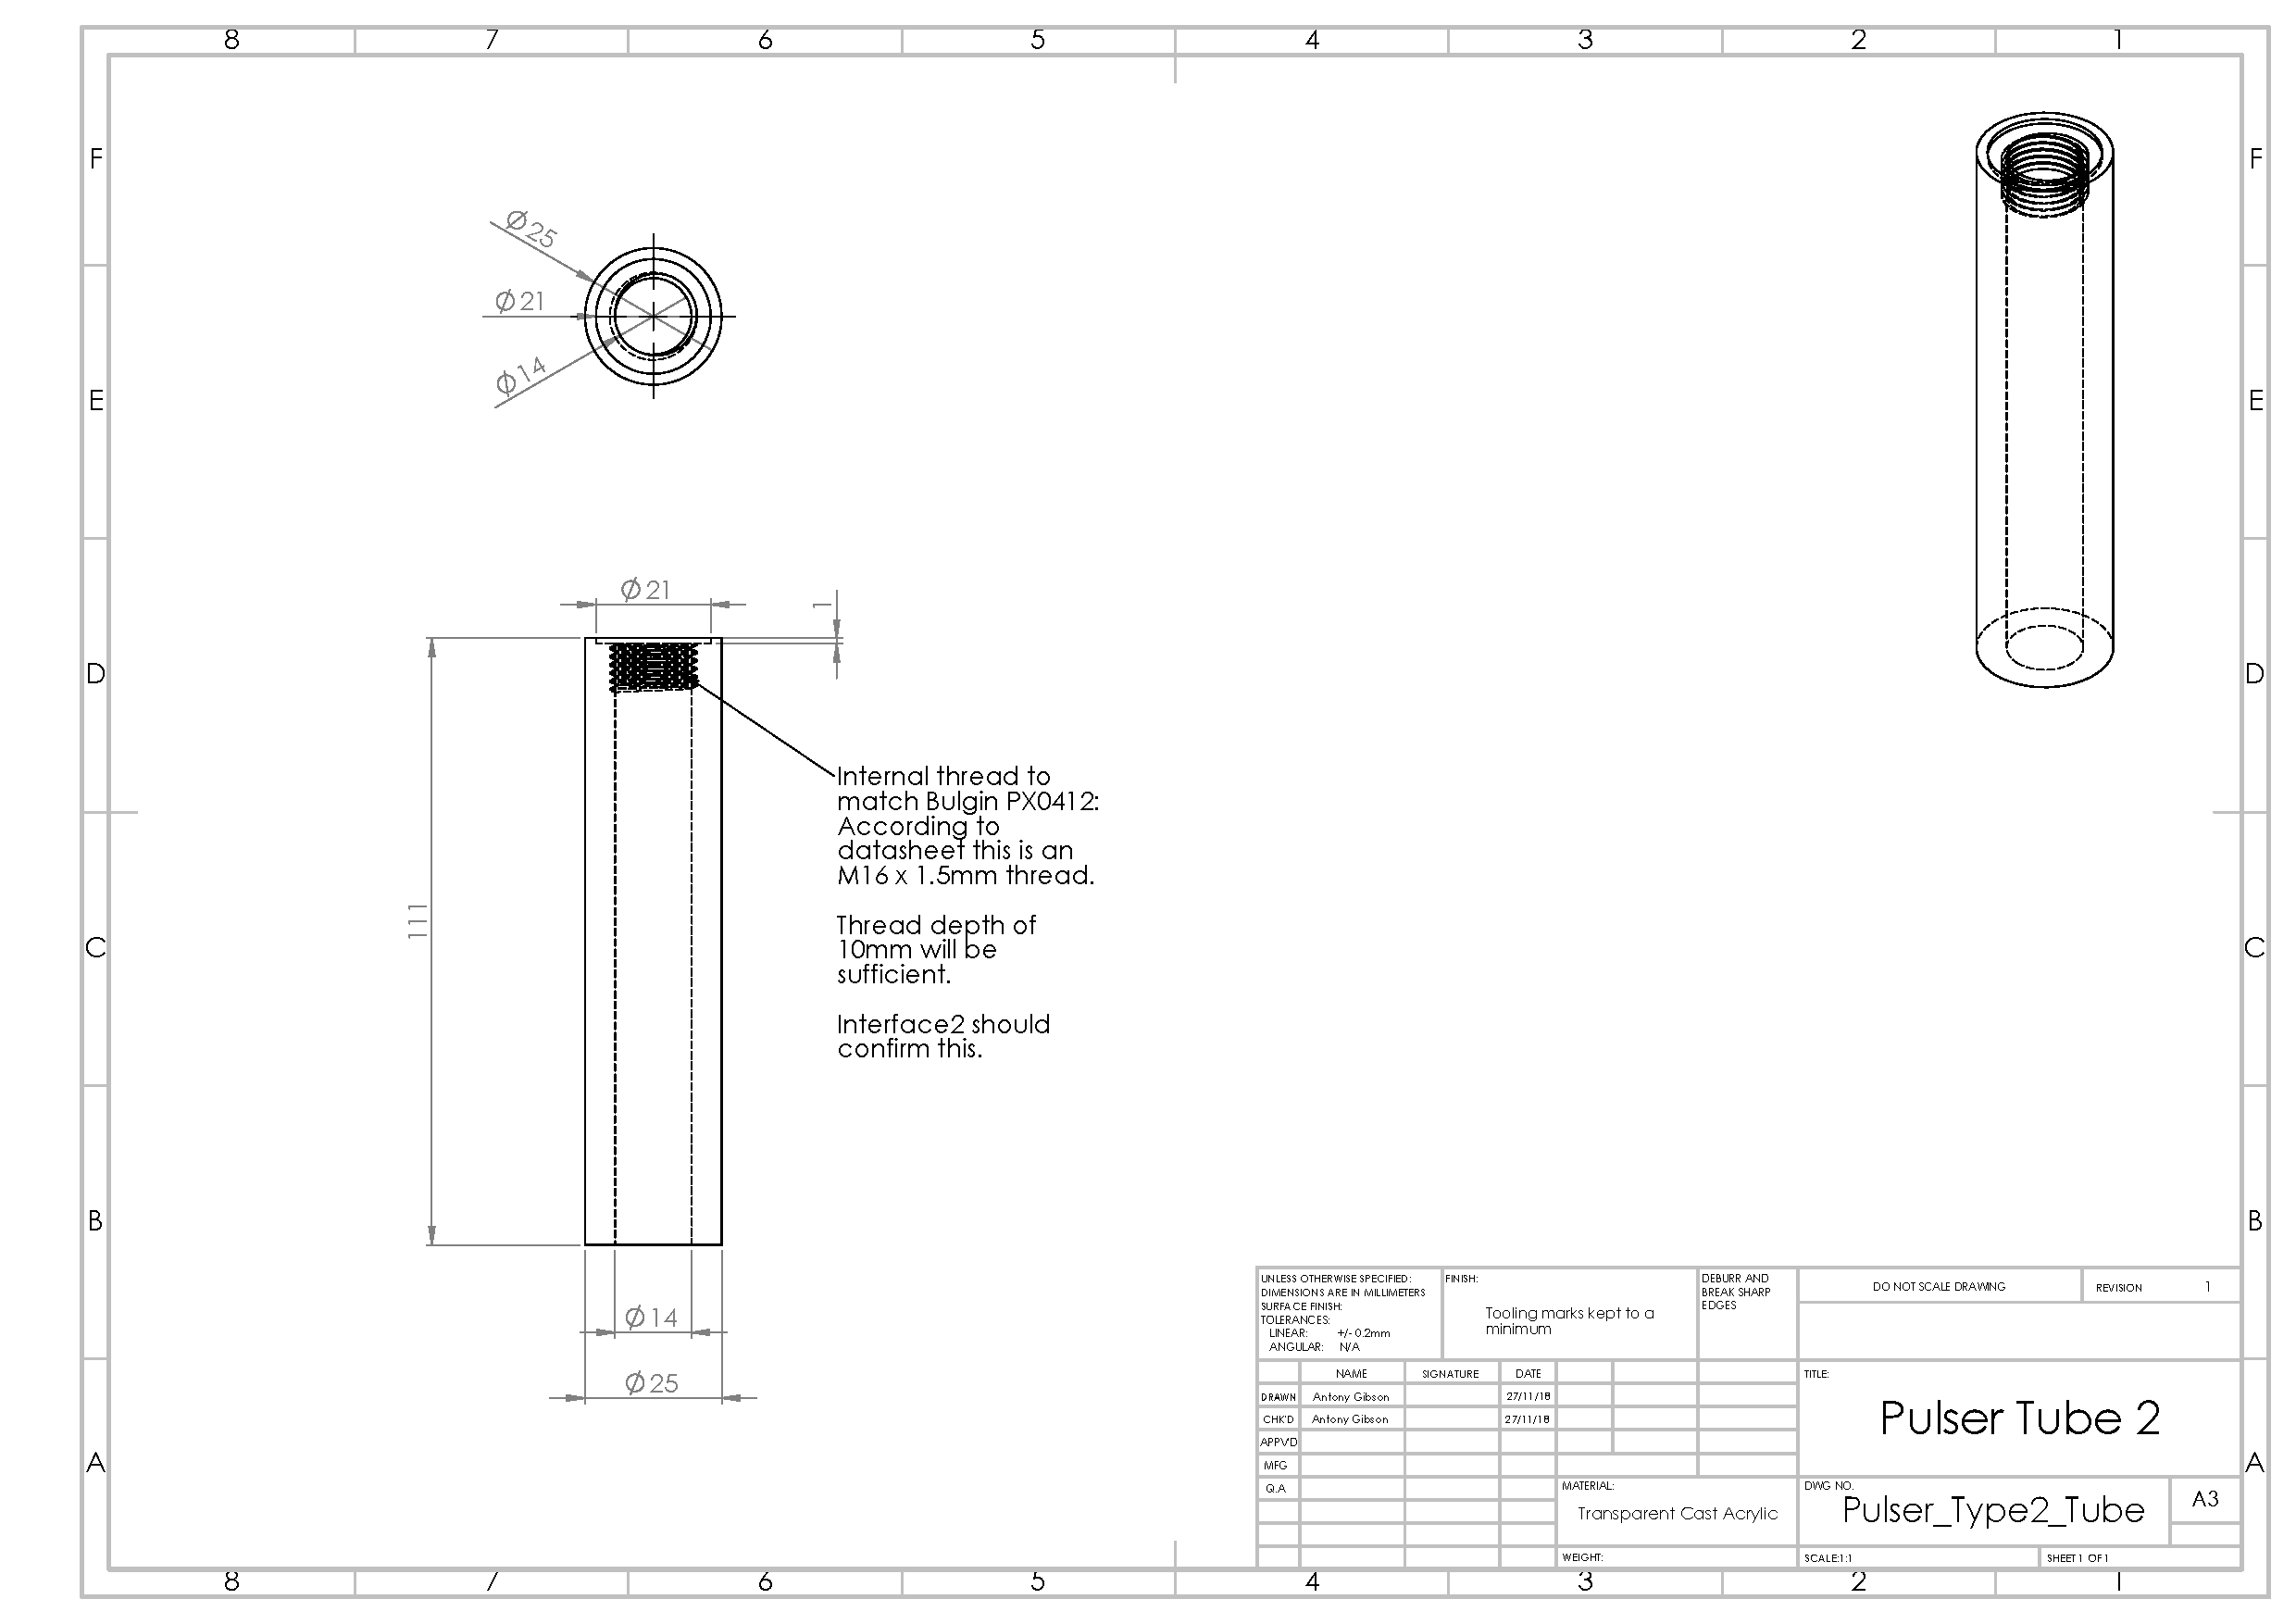
\includepdf{figures/Pulser_Type2_Tube.PDF}


%%%%%%%%%%%%%%%%%%%%%%%%%%%%%%%%%%%%%%%%%%%%%%%%%%
% To do list
%%%%%%%%%%%%%%%%%%%%%%%%%%%%%%%%%%%%%%%%%%%%%%%%%%
\ifdraft
\listoftodos
\fi
\end{document}